\subsection{Lab21:Filter taps}

%*********************
\begin{frame}{}

\pgfdeclareimage[width=\paperwidth,height=\paperheight]{bg}{imagenes/fondo_lab}
\setbeamertemplate{background}{\pgfuseimage{bg}}

\bfseries{\textrm{\LARGE Lab21\\ \Large Filter taps}}
\raggedright
\end{frame}
%*********************

\begin{frame}{Filter taps}
Taps
\begin{flushleft}
El parámetro Taps indica las secciones de un filtro FIR que emula un retardo con múltiples trayectos.
Uno de los parámetros más importantes  para este bloque son los coeficientes (taps) del filtro. Uno de los beneficios de implementación del bloque es que usted puede definir el filtro acoplado directamente en este bloque, lo que permite tener el filtro acoplado y la corrección de tiempo de muestreo de manera simultánea.
\end{flushleft}
\end{frame}

%*********************

\begin{frame}{Filter taps}
\begin{figure}[H]
\centering
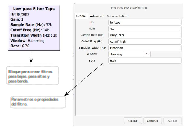
\includegraphics[width=.8\textwidth]{Modulaciones_digitales/lab21/pdf/lab21_1.pdf}
\end{figure}
\end{frame}
%*********************

\begin{frame}{Filter taps}
FIR Decimating
\begin{flushleft}
Este es un bloque que permite cargar toques de filtro desde un archivo (desde la herramienta de diseño de filtro).El nombre FIR viene de la manera en que el filtro afecta una señal. Una función impulso es una entrada bastante interesante, donde la señal es 0 siempre, excepto en un lugar donde tiene valor de 1.
\end{flushleft}
\end{frame}

%*********************

\begin{frame}{Filter taps}
\begin{figure}[H]
\centering
\vspace{-3mm}
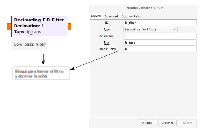
\includegraphics[width=\textwidth]{Modulaciones_digitales/lab21/pdf/lab21_2.pdf}
\end{figure}
\end{frame}

%*********************

\begin{frame}{Filter taps}
\begin{figure}[H]
\centering
\vspace{-3mm}
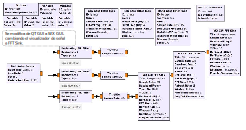
\includegraphics[width=\textwidth]{Modulaciones_digitales/lab21/pdf/lab21_3.pdf}
\end{figure}
\end{frame}
%*********************

\begin{frame}{Filter taps}
\begin{figure}[H]
\centering
\vspace{-3mm}
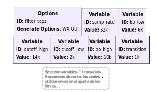
\includegraphics[width=\textwidth]{Modulaciones_digitales/lab21/pdf/lab21_4.pdf}
\end{figure}
\end{frame}

%*********************

\begin{frame}{Filter taps}
\begin{figure}[H]
\centering
\vspace{-3mm}
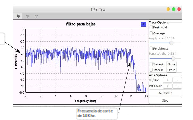
\includegraphics[width=\textwidth]{Modulaciones_digitales/lab21/pdf/lab21_5.pdf}
\end{figure}
\end{frame}

%*********************

\begin{frame}{Filter taps}
\begin{figure}[H]
\centering
\vspace{-3mm}
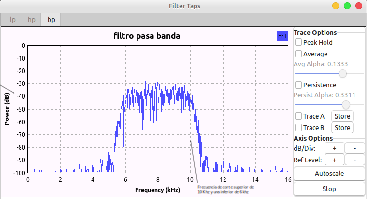
\includegraphics[width=\textwidth]{Modulaciones_digitales/lab21/pdf/lab21_6.pdf}
\end{figure}
\end{frame}




